\documentclass{TIJMUjiaoanLL}
\pagestyle{empty}


\begin{document}


%课程名称
\kecheng{生物信息学}
%课程内容
\neirong{基因组功能注释分析基础}
%教师姓名
\jiaoshi{伊现富}
%职称
\zhicheng{讲师}
%教学日期(格式:XXXX年XX月XX日XX时-XX时)
\riqi{2014年4月2日10时-12时}
%授课对象(格式:XXX系XXXX年级XX班(硕/本/专科))
\duixiang{生物医学工程学院2011级生信班(本)}
%听课人数
\renshu{27}
%授课方式
\fangshi{理论讲授}
%学时数
\xueshi{2}
%教材版本
\jiaocai{生物信息学(自编教材)}


%教案首页
\firstHeader
\maketitle
\thispagestyle{empty}

\mudi{
\begin{itemize}
  \item 掌握基因组的两种坐标系统;FASTA和BED格式;基因组坐标的常见逻辑运算。
  \item 熟悉GFF格式;不同操作系统中换行符的差异。
  \item 了解基因组的组装版本及常见版本间的对应关系;纯文本与格式化文本的区别;常见的文本编辑器。
  \item 自学VCF格式;基因组坐标的其他逻辑运算。
\end{itemize}
}

\fenpei{
\begin{itemize}
  \item (5')回顾与导入:回顾基因组注释中结构注释的知识,介绍功能注释的主要内容。
  \item (10')基因组组装版本:介绍基因组的组装版本、不同数据库中组装版本的命名及其对应关系。
  \item (15')基因组坐标系统:举例讲解0-based和1-based两种不同的基因组坐标系统及其各自的适用范围。
  \item (20')基因组注释常用格式:通过实例详细讲解FASTA和BED格式,简单介绍GFF格式,学生自学VCF格式。
  \item (10')文本文件与文本编辑器:介绍纯文本和格式化文本的区别,讲解不同操作系统中换行符的差异,推荐几个常用的文本编辑器。
  \item (35')基因组坐标的逻辑运算:通过图示和实例讲解交集、减法、补集等常用的基因组坐标逻辑运算。
  \item (5')总结与答疑:总结授课内容中的知识点与技能,解答学生疑问。
\end{itemize}
}

\zhongdian{
\begin{itemize}
  \item 重点:基因组的两种坐标系统,基因组注释中常用的BED格式,基因组坐标的逻辑运算。
  \item 难点:基因组坐标中的0-based坐标系统,基因组坐标的逻辑运算。
  \item 解决策略:通过形象化的图示、与集合运算等的类比解释基本概念,通过实例演算帮助学生理解记忆。
\end{itemize}
}

\waiyu{
\vspace*{-10pt}
\begin{multicols}{2}
基因组注释(genome annotation)

功能注释(functional annotation)

基因组组装版本(genome build)

坐标系统(coordinate system)

坐标转换(coordinate transform)

集合运算(set operation)
\end{multicols}
\vspace*{-10pt}
}

\fuzhu{
\begin{itemize}
  \item 多媒体:两种坐标系统、注释常用格式、逻辑运算等的示意图。
  \item 板书:两种坐标系统、FASTA和BED格式、逻辑运算的简单示例。
\end{itemize}
}

\sikao{
\vspace*{-10pt}
\begin{multicols}{2}
\begin{itemize}
  \item hg19和mm10分别代表什么含义?
  \item 举例说明基因组的两种坐标系统。
  \item BED格式前6列分别代表什么含义?
  \item 图示常见的基因组坐标逻辑运算。
  \item 不同操作系统的换行符有何区别?如何进行查看和转换?
\end{itemize}
\end{multicols}
\vspace*{-10pt}
}

\cankao{
\begin{itemize}
  \item UCSC FAQ(Frequently Asked Questions)
  \item Galaxy Wiki
  \item File formats on Wikipedia
\end{itemize}
}

\firstTail


%教案续页
\newpage
\otherHeader

\noindent
一、回顾与导入(5分钟)

基因组注释:\textcolor{red}{(回顾结构注释的相关内容,引出功能注释的主要工作)}
\begin{itemize}
  \item 结构注释:序列基本信息分析、寻找限制酶切位点、开放阅读框的预测、启动子和转录因子结合位点的分析、CpG 岛的识别、屏蔽重复序列、基因识别、……
  \item 功能注释
  \begin{itemize}
    \item 基础知识:组装版本、坐标系统、常用格式、坐标的逻辑运算、……
    \item 注释内容:变异位点的注释、富集分析、互作网络分析、进化分析、……
  \end{itemize}
\end{itemize}

\vspace*{0.2cm}
\noindent
二、基因组组装版本(10分钟)
\begin{enumerate}
  \item 基因组也有组装版本\textcolor{red}{(与操作系统、软件的版本变化进行类比)}
    \begin{itemize}
      \item We used DNA sequences from the human and mouse genome assemblies hg18 and mm9.
      \item The genome assemblies from which the sequences obtained were Dec 2011 (GRCm38/mm10), Feb 2009 (GRCh37/hg19) and Nov 2004 (Baylor3.4/rn4) for mouse, human and rat respectively.
  \end{itemize}
  \item 不同数据库采用不同的命名规则\textcolor{red}{(解释hg、mm、GRC等缩写的含义,帮助学生理解其命名)}
     \begin{itemize}
    \parpic[fr]{\includegraphics[width=8.5cm]{version.png}}
       \item NCBI:Build X
       \item Ensembl:NCBIX
       \item UCSC:hgX、mmX、……
     \end{itemize}
  \item 不同版本间存在对应关系
    \begin{itemize}
       \item hg19 = GRCh37; hg18 = NCBI Build 36.1
       \item mm10 = GRCm38; mm9 = NCBI Build 37
    \end{itemize}
\end{enumerate}

\vspace*{0.2cm}
\noindent
三、基因组坐标系统(15分钟)
\begin{enumerate}
  \item 基因组的坐标系统\textcolor{red}{(以数学中的坐标引出基因组的坐标)}
    \begin{figure}[h]
    \centering
      \includegraphics[width=8cm,height=1.6cm]{1d.png}
      \hspace*{0.2cm}
      \includegraphics[width=9.5cm]{dna.png}
    \end{figure}
    \parpic[fr]{\includegraphics[width=6cm,height=6.5cm]{firstFloor.jpg}}
    \begin{itemize}
      \item SNP, rs1800468, hg19: ''chr19:41860587''
      \item gene, SAMD11, hg19: ''chr1:861121-879961''
    \end{itemize}
  \item 坐标系统实例\textcolor{red}{(通过实例讲解两种坐标系统;类比英式和美式英语的first floor以及编程语言中的计数方式)}
    \begin{table}[h]
    %\centering
    \hspace*{2cm}
    \begin{tabular}{lcccccccc}
      \hline
      0-based index & 0 & 1 & 2 & 3 & 4 & 5 & 6 & 7\\
      \hline
      Sequence & A & A & T & T & G & G & C & C\\
      \hline
      1-based index & 1 & 2 & 3 & 4 & 5 & 6 & 7 & 8\\
      \hline
    \end{tabular}
  \end{table}
  \begin{itemize}
    \item 1-based(one-based, fully-closed):TG = [3,5]
    \item 0-based(zero-based, half-closed-half-open):TG = [4,5)
  \end{itemize}
  \item 坐标系统的适用范围\textcolor{red}{(引导学生思考两种坐标系统的优缺点)}
    \begin{itemize}
      \item 1-based:主要给研究人员肉眼查看的数据,如:GFF、VCF、SAM和Wiggle等格式以及DAS和UCSC的Genome Browser等工具
      \item 0-based:主要用于计算机程序处理的数据,如:BED、BAM和PSL等格式以及NCBI的dbSNP和UCSC的Table Browser等数据库与工具
    \end{itemize}
\end{enumerate}


\otherTail
\newpage
\otherHeader


\noindent
四、基因组注释常用格式(20分钟)

类似于多样的计算机数据需要多样的文件格式来存储一样,基因组数据类型的多样性导致了数据格式的多样性。\textcolor{red}{(通过计算机文件格式及格式间的转换引申出基因组数据格式)}
\begin{itemize}
  \item 序列 $\Rightarrow$ FASTA
  \parpic[fr]{\includegraphics[width=9cm]{fb.png}}
  \item 展示特征 $\Rightarrow$ BED(Browser Extensible Data)
  \item 特征 $\Rightarrow$ GFF(General Feature Format)
  \item 变异 $\Rightarrow$ VCF(Variant Call Format)
\end{itemize}

通过展示实例详细介绍FASTA、BED、GFF和VCF四种常用格式,讲解格式中每一列的含义,引导学生学会解析特定格式中的信息。同时强调它们都以纯文本形式进行存储的,可以使用常见的文本编辑器(Notepad++,Vim,Emacs)查看、编辑。
\begin{enumerate}
  \item FASTA格式\textcolor{red}{(强调FASTA与sequence之间的区别)}
    \begin{itemize}
      \item 首行:起始标识符“>”,ID,描述信息;其余行:具体的序列。
      \item IUB/IUPAC核酸代码:“N”代表任意一种核酸,“-”代表空位。
      \item IUB/IUPAC氨基酸代码:“X”代表任意一种氨基酸,“*”代表翻译终止,“-” 代表空位。
    \end{itemize}
  \item BED格式:3+9=12列(BED12),0-based。\textcolor{red}{引申出BED3,BED4,BED5和BED6。}
  \parpic[fr]{\includegraphics[width=8.5cm,height=3cm]{bed.png}}
    \begin{itemize}
      \item BED3:chrom, start, end\\ \hspace*{1.35cm} chr1\quad 11873\quad 14409
      \item BED4:chrom, start, end, name\\ \hspace*{1.35cm} chr1\quad 11873\quad 14409\quad uc001aaa.3
      \item BED5:chrom, start, end, name, score\\ \hspace*{1.35cm} chr1\quad 11873\quad 14409\quad uc001aaa.3\quad 0
      \item BED6:chrom, start, end, name, score, strand\\ \hspace*{1.35cm} chr1\quad 11873\quad 14409\quad uc001aaa.3\quad 0\quad +
    \end{itemize}
  \item GFF格式:1-based
  \parpic[fr]{\includegraphics[width=11cm,height=3.5cm]{gff.png}}
    \begin{itemize}
      \item 注释信息:以“\#\#”开头
      \item 特征信息:9列
    \end{itemize}
  \item VCF格式:1-based\textcolor{red}{(自学)}
    \begin{itemize}
      \item 元信息:以“\#\#”起始
      \item 标题行:以“\#”起始
      \item 数据行:8+1+N列
    \end{itemize}
\end{enumerate}

\vspace*{0.2cm}
\noindent
五、文本文件与文本编辑器(10分钟)
\begin{enumerate}
  \item 纯文本 vs. 格式化文本\textcolor{red}{(通过比较txt和doc这两种常见的文本文件格式,帮助学生理解纯文本和格式化文本的区别)}
  \item 换行符及其识别与转换
    \begin{itemize}
    \parpic[fr]{\includegraphics[width=7cm]{editor.png}}
      \item Windows:\verb|\r\n|(CR+LF,回车+换行),文件尾部直接EOF(文件结束标志)
      \item Unix:\verb|\n|(LF,仅有换行),文件最后一行也会增加该字符,然后才是EOF
      \item Mac:\verb|\r|(CR,仅有回车)
      \item Windows中的识别与转换:文本编辑器,如Notepad++
      \item Unix中的识别与转换:file识别,fromdos \& todos转换
    \end{itemize}
  \item 文本编辑器:Notepad++,Vim,Emacs,Sublime Text
\end{enumerate}


\otherTail
\newpage
\otherHeader


\noindent
六、基因组坐标的逻辑运算(35分钟)
\begin{enumerate}
  \item 集合运算与逻辑运算
    \begin{itemize}
      \item \textcolor{red}{类比数学中的集合运算}
      \item 以交集为例,讲解由集合运算转换到逻辑运算的过程
    \end{itemize}
    \begin{figure}[h]
      \centering
      \includegraphics[width=8cm]{set.png}
      \hspace*{1cm}
      \includegraphics[width=8cm]{setT.png}
    \end{figure}
  \item 基因组坐标逻辑运算\textcolor{red}{(先用示意图予以讲解,再辅以实例帮助记忆,最终理解其适用情况)}
    \begin{itemize}
    \parpic[fr]{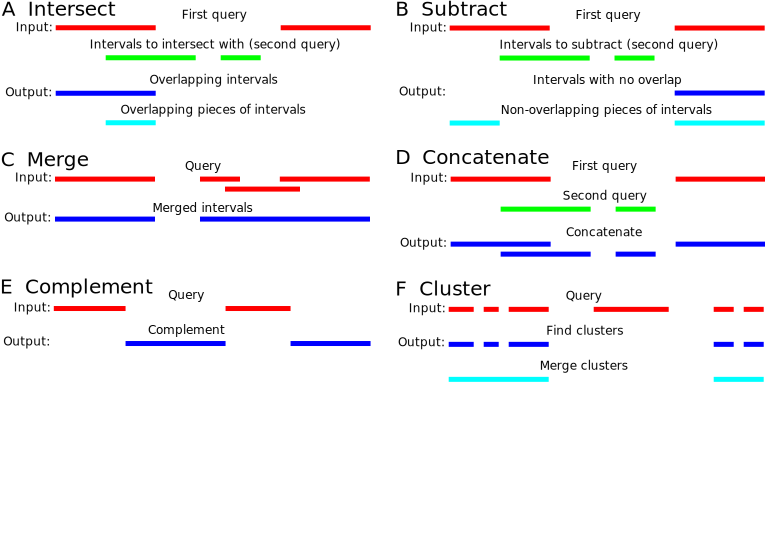
\includegraphics[width=9cm,height=5.5cm]{operation.png}}
      \item intersect,交集:保留重叠的坐标
      \item subtract,减法:去除重叠的坐标
      \item merge,合并:合并重叠的坐标
      \item concatenate,串联:合并多组坐标
      \item complement,补集:取坐标的补集
      \item cluster,聚类:聚合符合要求的坐标
      \item join,联合:根据坐标重叠把两组记录对应起来
      \item coverage, flank, closest, slop, window, \ldots \textcolor{red}{(学生自学)}
    \end{itemize}
\end{enumerate}

\vspace*{0.2cm}
\noindent
七、总结与答疑(5分钟)
\begin{enumerate}
  \item 知识点
    \begin{itemize}
    \parpic[fr]{\includegraphics[width=9cm,height=7cm]{join.png}}
      \item 基因组组装版本:命名规则,对应关系
      \item 两种基因组坐标系统:1-based,0-based
      \item 四种注释常用格式:FASTA,BED,GFF,VCF
      \item 坐标的逻辑运算:intersect,subtract,merge,concatenate,complement,cluster,join
    \end{itemize}
  \item 技能
    \begin{itemize}
      \item 纯文本与格式化文本
      \item 不同操作系统中的换行符
      \item 文本编辑器:Notepad++, Vim, Emacs
    \end{itemize}
\end{enumerate}


\otherTail


\end{document}

